% Original fixture. Historical reported figures; questions and diagrams are original.
% Source: NVIDIA FY2025 earnings release, 26 February 2025 (linked on final slide).
\documentclass[11pt,aspectratio=169]{beamer}
\usetheme{Madrid}
\usecolortheme{seahorse}
\usepackage{booktabs,pgfplots}
\pgfplotsset{compat=1.18}
\setbeamercolor{structure}{fg=teal!70!black}
\setbeamertemplate{navigation symbols}{}
\title[NVIDIA FY2025]{Growth, concentration, and the next question}
\subtitle{NVIDIA FY2025 performance review}
\author[Research workshop]{An original equity-research teaching case}
\institute[Teaching case]{Historical reporting exercise}
\date[FY2025]{Fiscal year ended 26 January 2025}
\begin{document}
\begin{frame}[plain]\titlepage\end{frame}
\section{Decision brief}
\begin{frame}{The result is strong; the next question is durability}
\begin{columns}[T,onlytextwidth]
\begin{column}{.31\textwidth}\begin{block}{Scale}\centering\LARGE\$130.5bn\par\normalsize FY2025 revenue\end{block}\end{column}
\begin{column}{.31\textwidth}\begin{block}{Growth}\centering\LARGE114\%\par\normalsize year over year\end{block}\end{column}
\begin{column}{.31\textwidth}\begin{block}{Profitability}\centering\LARGE75.0\%\par\normalsize GAAP gross margin\end{block}\end{column}
\end{columns}
\medskip
\alert{Discussion:} which of these indicators is most useful for judging repeatability?
\note{Ask participants to choose a metric before showing the trend. This is an analytical exercise, not company guidance.}
\end{frame}
\begin{frame}{A common scale makes the revenue change visible}
\begin{columns}[c]
\begin{column}{.59\textwidth}
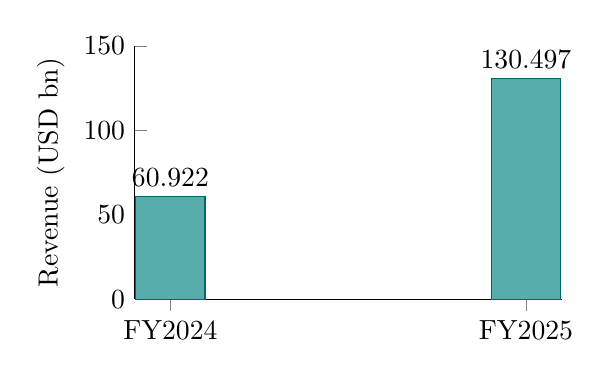
\begin{tikzpicture}
\begin{axis}[width=7cm,height=4.8cm,ybar,bar width=25pt,ymin=0,ymax=150,
 symbolic x coords={FY2024,FY2025},xtick=data,ylabel={Revenue (USD bn)},nodes near coords,
 axis lines*=left,ytick={0,50,100,150},
 every node near coord/.append style={/pgf/number format/fixed,/pgf/number format/precision=3,/pgf/number format/fixed zerofill}]
\addplot[fill=teal!65,draw=teal!80!black] coordinates {(FY2024,60.922) (FY2025,130.497)};
\end{axis}
\end{tikzpicture}
\end{column}
\begin{column}{.37\textwidth}
\begin{exampleblock}{Read the chart}
The axis starts at zero. Labels retain three decimal places to connect to the reported USD-million table.
\end{exampleblock}
\end{column}
\end{columns}
\end{frame}
\section{Quality of the result}
\begin{frame}{Keep GAAP comparisons on the same basis}
\begin{table}
\centering
\begin{tabular}{lrr}
\toprule
Metric & FY2024 & FY2025\\\midrule
Revenue (USD bn) & 60.922 & 130.497\\
Operating income (USD bn) & 32.972 & 81.453\\
Net income (USD bn) & 29.760 & 72.880\\
Gross margin & 72.7\% & 75.0\%\\\bottomrule
\end{tabular}
\caption{Reported annual GAAP figures; amounts converted from USD millions.}
\end{table}
\end{frame}
\begin{frame}{Separate a reported fact from an analyst inference}
\begin{description}
\item[Fact] FY2025 Data Center revenue was USD115.2bn.
\item[Calculation] Rounded segment revenue divided by total revenue is about 88\%.\footnote{Computed from rounded segment revenue and the reported annual total.}
\item[Inference] A segment-specific demand shock could matter disproportionately.
\end{description}
\pause
\begin{alertblock}{Question for the next review}
What evidence would distinguish a temporary purchasing cycle from sustained end demand?
\end{alertblock}
\end{frame}
\begin{frame}{A scenario is a sensitivity, not a forecast}
\framesubtitle{Deliberately hypothetical: hold everything except revenue and margin fixed}
Let revenue be $R$ and gross margin be $m$. Gross profit is $G=Rm$.
\[
 \Delta G=m\,\Delta R+R\,\Delta m+\Delta R\,\Delta m.
\]
\begin{itemize}[<+->]
\item A revenue change and a margin change are different economic mechanisms.
\item A two-variable sensitivity prevents the same shock being counted twice.
\item This identity is not an earnings forecast or a valuation model.
\end{itemize}
\end{frame}
\section{Actions}
\begin{frame}{Three questions for management discussion}
\begin{enumerate}
\item \textbf{Demand:} what observation would invalidate the base case?
\item \textbf{Execution:} which operating constraint is binding?
\item \textbf{Evidence:} what should be observable before the next reporting date?
\end{enumerate}
\bigskip
\begin{block}{Meeting output}
Assign an owner, an observable indicator, and a date to each question.
\end{block}
\end{frame}
\appendix
\begin{frame}{Source and scope}
\small
\begin{thebibliography}{9}
\bibitem{nvda} NVIDIA. \emph{Financial Results for Fourth Quarter and Fiscal 2025}. 26 February 2025.
\href{https://nvidianews.nvidia.com/news/nvidia-announces-financial-results-for-fourth-quarter-and-fiscal-2025}{Official earnings release and GAAP tables}.
\end{thebibliography}
\medskip
Original educational slides; not issued by NVIDIA. Historical facts are distinguished from original calculations and hypothetical sensitivities. Per-share measures are omitted to avoid mixing split-adjusted bases.
\end{frame}
\end{document}
